\documentclass{article}
\usepackage[english]{babel}
\usepackage[utf8]{inputenc}
\usepackage[english]{babel}
\usepackage[a4paper, total={7.25in, 9.5in}]{geometry}
\usepackage{tikz-feynman}
\tikzfeynmanset{compat=1.0.0} 
\usepackage{subcaption}
\usepackage{float}
\floatplacement{figure}{H}
\usepackage{simpler-wick}
\usepackage{mathrsfs}  
\usepackage{dsfont}
\usepackage{relsize}
\usepackage{tikz-cd}
\DeclareMathAlphabet{\mathdutchcal}{U}{dutchcal}{m}{n}

\usepackage{cancel}



\newcommand{\field}{\hat{\Phi}}
\newcommand{\dfield}{\hat{\Phi}^\dagger}
 
\usepackage{amsthm, amssymb, amsmath, centernot}
\usepackage{slashed}
\newcommand{\notimplies}{%
  \mathrel{{\ooalign{\hidewidth$\not\phantom{=}$\hidewidth\cr$\implies$}}}}
 
\renewcommand\qedsymbol{$\square$}
\newcommand{\cont}{$\boxtimes$}
\newcommand{\divides}{\mid}
\newcommand{\ndivides}{\centernot \mid}

\newcommand{\Integers}{\mathbb{Z}}
\newcommand{\Natural}{\mathbb{N}}
\newcommand{\Complex}{\mathbb{C}}
\newcommand{\Zplus}{\mathbb{Z}^{+}}
\newcommand{\Primes}{\mathbb{P}}
\newcommand{\Q}{\mathbb{Q}}
\newcommand{\R}{\mathbb{R}}
\newcommand{\ball}[2]{B_{#1} \! \left(#2 \right)}
\newcommand{\Rplus}{\mathbb{R}^+}
\renewcommand{\Re}[1]{\mathrm{Re}\left[ #1 \right]}
\renewcommand{\Im}[1]{\mathrm{Im}\left[ #1 \right]}
\newcommand{\Op}{\mathcal{O}}

\newcommand{\invI}[2]{#1^{-1} \left( #2 \right)}
\newcommand{\End}[1]{\text{End}\left( A \right)}
\newcommand{\legsym}[2]{\left(\frac{#1}{#2} \right)}
\renewcommand{\mod}[3]{\: #1 \equiv #2 \: \mathrm{mod} \: #3 \:}
\newcommand{\nmod}[3]{\: #1 \centernot \equiv #2 \: mod \: #3 \:}
\newcommand{\ndiv}{\hspace{-4pt}\not \divides \hspace{2pt}}
\newcommand{\finfield}[1]{\mathbb{F}_{#1}}
\newcommand{\finunits}[1]{\mathbb{F}_{#1}^{\times}}
\newcommand{\ord}[1]{\mathrm{ord}\! \left(#1 \right)}
\newcommand{\quadfield}[1]{\Q \small(\sqrt{#1} \small)}
\newcommand{\vspan}[1]{\mathrm{span}\! \left\{#1 \right\}}
\newcommand{\galgroup}[1]{Gal \small(#1 \small)}
\newcommand{\bra}[1]{\left| #1 \right>}
\newcommand{\Oa}{O_\alpha}
\newcommand{\Od}{O_\alpha^{\dagger}}
\newcommand{\Oap}{O_{\alpha '}}
\newcommand{\Odp}{O_{\alpha '}^{\dagger}}
\newcommand{\im}[1]{\mathrm{im} \: #1}
\renewcommand{\ker}[1]{\mathrm{ker} \: #1}
\newcommand{\ket}[1]{\left| #1 \right>}
\renewcommand{\bra}[1]{\left< #1 \right|}
\newcommand{\inner}[2]{\left< #1 | #2 \right>}
\newcommand{\expect}[2]{\left< #1 \right| #2 \left| #1 \right>}
\renewcommand{\d}[1]{ \mathrm{d}#1 \:}
\newcommand{\dn}[2]{ \mathrm{d}^{#1} #2 \:}
\newcommand{\deriv}[2]{\frac{\d{#1}}{\d{#2}}}
\newcommand{\nderiv}[3]{\frac{\dn{#1}{#2}}{\d{#3^{#1}}}}
\newcommand{\pderiv}[2]{\frac{\partial{#1}}{\partial{#2}}}
\newcommand{\fderiv}[2]{\frac{\delta #1}{\delta #2}}
\newcommand{\parsq}[2]{\frac{\partial^2{#1}}{\partial{#2}^2}}
\newcommand{\topo}{\mathcal{T}}
\newcommand{\base}{\mathcal{B}}
\renewcommand{\bf}[1]{\mathbf{#1}}
\renewcommand{\a}{\hat{a}}
\newcommand{\adag}{\hat{a}^\dagger}
\renewcommand{\b}{\hat{b}}
\newcommand{\bdag}{\hat{b}^\dagger}
\renewcommand{\c}{\hat{c}}
\newcommand{\cdag}{\hat{c}^\dagger}
\newcommand{\hamilt}{\hat{H}}
\renewcommand{\L}{\hat{L}}
\newcommand{\Lz}{\hat{L}_z}
\newcommand{\Lsquared}{\hat{L}^2}
\renewcommand{\S}{\hat{S}}
\renewcommand{\empty}{\varnothing}
\newcommand{\J}{\hat{J}}
\newcommand{\lagrange}{\mathcal{L}}
\newcommand{\dfourx}{\mathrm{d}^4x}
\newcommand{\meson}{\phi}
\newcommand{\dpsi}{\psi^\dagger}
\newcommand{\ipic}{\mathrm{int}}
\newcommand{\tr}[1]{\mathrm{tr} \left( #1 \right)}
\newcommand{\C}{\mathbb{C}}
\newcommand{\CP}[1]{\mathbb{CP}^{#1}}
\newcommand{\Vol}[1]{\mathrm{Vol}\left(#1\right)}

\newcommand{\Tr}[1]{\mathrm{Tr}\left( #1 \right)}
\newcommand{\Charge}{\hat{\mathbf{C}}}
\newcommand{\Parity}{\hat{\mathbf{P}}}
\newcommand{\Time}{\hat{\mathbf{T}}}
\newcommand{\Torder}[1]{\mathbf{T}\left[ #1 \right]}
\newcommand{\Norder}[1]{\mathbf{N}\left[ #1 \right]}
\newcommand{\Znorm}{\mathcal{Z}}
\newcommand{\EV}[1]{\left< #1 \right>}
\newcommand{\interact}{\mathrm{int}}
\newcommand{\covD}{\mathcal{D}}
\newcommand{\conj}[1]{\overline{#1}}

\newcommand{\SO}[2]{\mathrm{SO}(#1, #2)}
\newcommand{\SU}[2]{\mathrm{SU}(#1, #2)}

\newcommand{\anticom}[2]{\left\{ #1 , #2 \right\}}


\newcommand{\pathd}[1]{\! \mathdutchcal{D} #1 \:}

\renewcommand{\theenumi}{(\alph{enumi})}


\renewcommand{\theenumi}{(\alph{enumi})}

\newcommand{\atitle}[1]{\title{% 
	\large \textbf{Physics GR8048 Quantum Field Theory II
	\\ Assignment \# #1} \vspace{-2ex}}
\author{Benjamin Church }
\maketitle}

\newcommand{\atitleIII}[1]{\title{% 
	\large \textbf{Physics GR8049 Quantum Field Theory III
	\\ Assignment \# #1} \vspace{-2ex}}
\author{Benjamin Church }
\maketitle}

\theoremstyle{definition}
\newtheorem{theorem}{Theorem}[section]
\newtheorem{definition}{definition}[section]
\newtheorem{lemma}[theorem]{Lemma}
\newtheorem{proposition}[theorem]{Proposition}
\newtheorem{corollary}[theorem]{Corollary}
\newtheorem{example}[theorem]{Example}
\newtheorem{remark}[theorem]{Remark}

\usepackage{relsize}
\begin{document}



\section*{Mass Renormalization}


\section*{1-Loop Mass $\psi$}
\begin{equation*}
\feynmandiagram [horizontal = a to b, layered layout, baseline = (a)] {
	i1 -- [fermion, momentum'=$p$] a -- [fermion, momentum'=$p - k$] b -- [fermion, momentum'=$p$] f1,
	a -- [scalar, half left, momentum=$k$] b
	};
\quad
\mathlarger{+}
\quad 	
\feynmandiagram [horizontal = a to b, layered layout, baseline = (a)] {
	i1 -- [fermion, momentum'=$p$] a [crossed dot, label = \(- i c_2\)] -- [fermion, momentum'=$p$] b
	};	
\end{equation*}

\section*{1-Loop Mass $\phi$}

\begin{equation*}
\feynmandiagram [horizontal = a to b, layered layout, baseline = (a)] {
	i1 -- [scalar, momentum'=$p$] a -- [fermion, half right, momentum'=$p + k$] b -- [scalar, momentum'=$p$] f1,
	b -- [fermion, half right, momentum'=$k$] a
	};
\quad
\mathlarger{+}
\quad 	
\feynmandiagram [horizontal = a to b, layered layout, baseline = (a)] {
	i1 -- [scalar, momentum'=$p$] a [crossed dot, label = \(- i c_3\)] -- [scalar, momentum'=$p$] b
	};	
\end{equation*}

\section*{Vertex Function}

\begin{equation*}
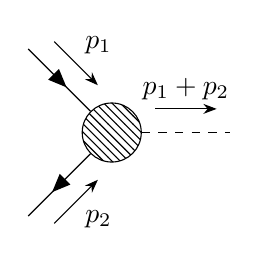
\begin{tikzpicture}[baseline = (b)]
\begin{feynman}
\vertex [blob] (b) {};
\vertex [above left=of b] (a);
\vertex [below left=of b] (c);
\vertex [right=of b] (d);
\diagram* {
(a) -- [fermion, momentum = $p_1$] (b) -- [fermion, rmomentum = $p_2$] (c),
(b) -- [scalar, momentum=$p_1 + p_2$] (d)
};
\end{feynman}
\end{tikzpicture}
 = - i \Gamma(p_1, p_2)
\end{equation*}

\begin{equation*}
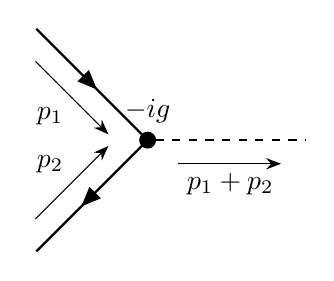
\begin{tikzpicture}[baseline = (a)]
\begin{feynman}[large]
\vertex [dot, label = $-ig$] (a) {};
\vertex [below left=of a] (b);
\vertex [above left=of a] (c);
\vertex [right=of a] (d);
\diagram* {
(a) -- [fermion, rmomentum'=$p_2$] (b),
(c) -- [fermion, momentum'=$p_1$] (a),
(a) -- [scalar, momentum'=$p_1 + p_2$] (d)
};
\end{feynman}
\end{tikzpicture}
\quad
\mathlarger{+}
\quad 	
\feynmandiagram [horizontal = a to b, baseline = (a)] {
	i1 -- [fermion, momentum'=$p_1$] t1 -- [fermion, momentum=$p_1 - k$] a,
	a -- [fermion, rmomentum=$p_2 + k$] t2 -- [fermion, rmomentum'=$p_2$] i2, 
	t1 -- [scalar, momentum'=$k$] t2,
	a -- [scalar, momentum'=$p_1 + p_2$ ] b
	};
\quad
\mathlarger{+}
\quad 	
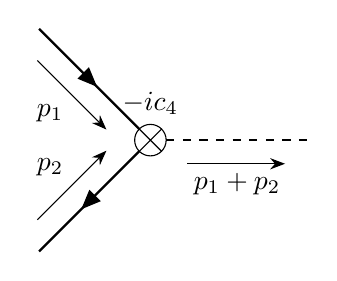
\begin{tikzpicture}[baseline = (a)]
\begin{feynman}[large]
\vertex [crossed dot, label = $-ic_4$] (a) {};
\vertex [below left=of a] (b);
\vertex [above left=of a] (c);
\vertex [right=of a] (d);
\diagram* {
(a) -- [fermion, rmomentum'=$p_2$] (b),
(c) -- [fermion, momentum'=$p_1$] (a),
(a) -- [scalar, momentum'=$p_1 + p_2$] (d)
};
\end{feynman}
\end{tikzpicture}
\end{equation*}

\section*{All the Diagrams}

\begin{equation*}
\feynmandiagram [baseline=(b.base), horizontal=a to b] {
i1 -- [fermion] a [blob],
a -- [fermion] i2,
f1 -- [fermion] b -- [fermion] f2,
a -- [scalar] b
};
\quad
+ 
\quad
\feynmandiagram [baseline = (l.base), vertical =b to d] {
a -- [fermion] b -- [fermion] c,
b -- [scalar] l [blob],
l -- [scalar] d,
f2 -- [fermion] d -- [fermion] f1,
};
\quad
+
\quad
\feynmandiagram [baseline=(b.base), horizontal=b to a] {
i1 -- [fermion] a [blob] ,
a -- [fermion] i2,
f1 -- [fermion] b -- [fermion] f2,
a -- [scalar] b
};
\end{equation*}

\begin{equation*}
\feynmandiagram [baseline=(b.base), vertical=a to b] {
i1 -- [fermion] a [blob],
i2 -- [fermion] a,
f1 -- [fermion] b -- [fermion] f2,
a -- [scalar] b
};
\quad
+ 
\quad
\feynmandiagram [baseline = (l.base), horizontal =b to d] {
a -- [fermion] b -- [fermion] c,
b -- [scalar] l [blob],
l -- [scalar] d,
f2 -- [fermion] d -- [fermion] f1,
};
\quad
+
\quad
\feynmandiagram [baseline=(a.base), vertical=b to a] {
i1 -- [fermion] a [blob] ,
i2 -- [fermion] a,
f1 -- [fermion] b -- [fermion] f2,
a -- [scalar] b
};
\end{equation*}
\begin{equation*}
\feynmandiagram [horizontal=s1 to s2] {
i1 -- [fermion] s1 -- [fermion] s2 -- [fermion] f1,
f2 -- [fermion] s3 -- [fermion] s4 -- [fermion] i2,
s1 -- [scalar] s4,
s2 -- [scalar] s3
};
\quad 
\quad 
\feynmandiagram [horizontal=s1 to s4] {
i1 -- [fermion] s1 -- [fermion] s2 -- [fermion] i2,
f1 -- [fermion] s3 -- [fermion] s4 -- [fermion] f2,
s1 -- [scalar] s4,
s2 -- [scalar] s3
};
\quad 
\quad
\begin{tikzpicture}
\begin{feynman}
\vertex (i1) ;
\vertex [below right=of i1] (s1);
\vertex [right=of s1] (s2);
\vertex [below=of s2] (s3);
\vertex [left=of s3] (s4);
\vertex [below left=of s4] (i2);
\vertex [below right=of s3] (f2);
\vertex [above right=of s2] (f1);
\diagram* {
(i1) -- [fermion] (s1) -- [fermion] (s4) -- [fermion] (i2),
(f2) -- [fermion] (s3) -- [fermion] (s2) -- [fermion] (f1),
(s1) -- [scalar] (s3)
(s2) -- [scalar] (s4)
};
\end{feynman}
\end{tikzpicture}
\quad 
\quad
\begin{tikzpicture}
\begin{feynman}
\vertex (i1) ;
\vertex [below right=of i1] (s1);
\vertex [right=of s1] (s2);
\vertex [below=of s2] (s3);
\vertex [left=of s3] (s4);
\vertex [below left=of s4] (i2);
\vertex [below right=of s3] (f2);
\vertex [above right=of s2] (f1);
\diagram* {
(i1) -- [fermion] (s1) -- [fermion] (s2) -- [fermion] (f1),
(f2) -- [fermion] (s3) -- [fermion] (s4) -- [fermion] (i2),
(s1) -- [scalar] (s3)
(s2) -- [scalar] (s4)
};
\end{feynman}
\end{tikzpicture}
\end{equation*}


\subsection{The Scattering Cross Amplitudes}

We now have all the tools necessary to compute the scattering cross section for the $\psi \bar{\psi} \to \psi \bar{\psi}$ process at the one-loop level. Following the LSZ reduction formula, we need only consider connected amputated diagrams. The first step is to properly organize the Feynman diagrams to simplify computations. There are two tree-level diagrams, ten one-loop diagrams, and six counterterm diagrams. I will organize these diagrams into classes of diagrams that ``look like'' each of the schematics,

(PUT IN DIAGRAM LIST)

We must consider each class of diagrams. 

\subsubsection{Class (a)}
We must consider the class of diagrams,

\begin{equation*}
\begin{tikzpicture}[baseline = (b)]
\begin{feynman}[large]
\vertex [blob] (b) {};
\vertex [above left=of b] (a);
\vertex [below left=of b] (c);
\vertex [right=of b] (d);
\vertex [above right=of d] (e);
\vertex [below right=of d] (f);
\diagram* {
(a) -- [fermion, momentum = $p_1$] (b) -- [fermion, rmomentum = $p_2$] (c),
(b) -- [scalar, momentum=$p_1 + p_2$] (d)
(e) -- [fermion, rmomentum' = $p_1'$] (d) -- [fermion, momentum' = $p_2'$] (f)
};
\end{feynman}
\end{tikzpicture}
\quad
\mathlarger{=}
\quad 	
\feynmandiagram [horizontal = a to b, baseline = (a)] {
	a -- [fermion] t1 -- [fermion, rmomentum=$p_1$] i1,
	i2 -- [fermion, momentum=$p_2$] t2 -- [fermion] a, 
	t1 -- [scalar] t2,
	a -- [scalar] b,
	o1 -- [fermion, rmomentum=$p_2'$] b -- [fermion, momentum=$p_1'$] o2
	};
\quad
\mathlarger{+}
\quad 	
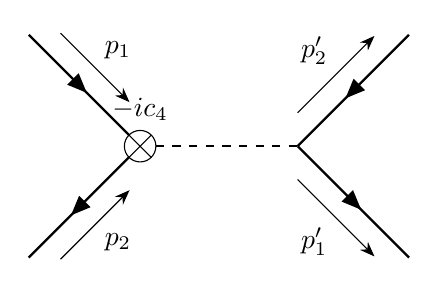
\begin{tikzpicture}[baseline = (a)]
\begin{feynman}[large]
\vertex [crossed dot, label = $-ic_4$] (a) {};
\vertex [below left=of a] (b);
\vertex [above left=of a] (c);
\vertex [right=of a] (d);
\vertex [above right=of d] (o1);
\vertex [below right=of d] (o2);
\diagram* {
(a) -- [fermion, rmomentum=$p_2$] (b),
(c) -- [fermion, momentum=$p_1$] (a),
(a) -- [scalar] (d),
(o1) -- [fermion, rmomentum'=$p_2'$] (d) -- [fermion, momentum'=$p_1'$] (o2)
};
\end{feynman}
\end{tikzpicture}
\end{equation*}
which gives an amplitude,
\[ i\mathcal{M}_a = -i \tilde{\Gamma}(p_1, p_2) \cdot \frac{i}{(p_1 + p_2)^2   - m^2} \]

\subsubsection{Class (b)}
Vertical middle loop diagrams look like,
\begin{equation*}
\feynmandiagram [baseline = (l), vertical = b to l] {
a -- [fermion, rmomentum=$p_2'$] b -- [fermion, rmomentum=$p_2$] c,
b -- [scalar] l [blob],
l -- [scalar] d,
f2 -- [fermion, momentum=$p_1$] d -- [fermion, momentum=$p_1'$] f1,
};
\quad
=
\quad
\feynmandiagram [baseline = (l2.base), vertical =b to d] {
a -- [fermion, rmomentum=$p_2'$] b -- [fermion, rmomentum=$p_2$] c,
b -- [scalar] l1 
-- [fermion, half left, looseness=1.5] l2 
--[fermion, half left, looseness=1.5] l1,
l2 -- [scalar] d,
f2 -- [fermion, momentum=$p_1$] d -- [fermion, momentum=$p_1'$] f1,
};
\quad 
+
\quad
\feynmandiagram [baseline = (l.base), vertical =b to d] {
a -- [fermion, rmomentum=$p_2'$] b -- [fermion, rmomentum=$p_2$] c,
b -- [scalar] l [crossed dot],
l -- [scalar] d,
f2 -- [fermion, momentum=$p_1$] d -- [fermion, momentum=$p_1'$] f1,
};
\end{equation*}
which give an amplitude,
\[ i\mathcal{M}_b =  \frac{i}{(p_1 - p_1')^2   - m^2} \cdot\left[ -i \Sigma(p_1 - p_1') \right] \cdot \frac{i}{(p_1 - p_1')^2   - m^2}  \]
\subsubsection{Class (c)}
The next set of diagrams look like,
\begin{equation*}
\begin{tikzpicture}[baseline = (b)]
\begin{feynman}[large]
\vertex (b);
\vertex [above left=of b] (a);
\vertex [below left=of b] (c);
\vertex [right=of b, blob] (d) {};
\vertex [above right=of d] (e);
\vertex [below right=of d] (f);
\diagram* {
(a) -- [fermion, momentum = $p_1$] (b) -- [fermion, rmomentum = $p_2$] (c),
(b) -- [scalar, momentum=$p_1 + p_2$] (d)
(e) -- [fermion, rmomentum' = $p_1'$] (d) -- [fermion, momentum' = $p_2'$] (f)
};
\end{feynman}
\end{tikzpicture}
\quad
\mathlarger{=}
\quad 	
\feynmandiagram [horizontal = b to a, baseline = (a)] {
	a -- [fermion] t1 -- [fermion, momentum=$p_1'$] i1,
	i2 -- [fermion, rmomentum=$p_2'$] t2 -- [fermion] a, 
	t1 -- [scalar] t2,
	a -- [scalar] b,
	o1 -- [fermion, momentum=$p_2$] b -- [fermion, rmomentum=$p_1$] o2
	};
\quad
\mathlarger{+}
\quad 	
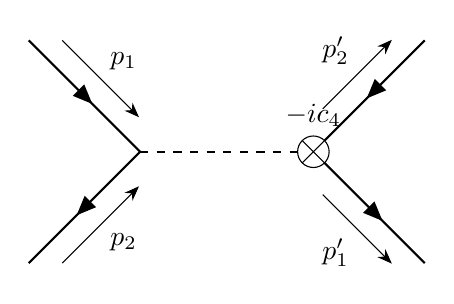
\begin{tikzpicture}[baseline = (a)]
\begin{feynman}[large]
\vertex (a);
\vertex [below left=of a] (b);
\vertex [above left=of a] (c);
\vertex [right=of a, crossed dot, label = $-ic_4$] (d) {};
\vertex [above right=of d] (o1);
\vertex [below right=of d] (o2);
\diagram* {
(a) -- [fermion, rmomentum=$p_2$] (b),
(c) -- [fermion, momentum=$p_1$] (a),
(a) -- [scalar] (d),
(o1) -- [fermion, rmomentum'=$p_2'$] (d) -- [fermion, momentum'=$p_1'$] (o2)
};
\end{feynman}
\end{tikzpicture}
\end{equation*}
which gives an amplitude,
\[ i\mathcal{M}_c = -i \tilde{\Gamma}(p_1', p_2') \cdot \frac{i}{(p_1 + p_2)^2   - m^2} \]


\subsubsection{Class (d)}
These diagrams are similar,
\begin{center}
\feynmandiagram [baseline=(b.base), vertical=a to b] {
i1 -- [fermion, rmomentum=$p_1'$] a [blob],
i2 -- [fermion, momentum'=$p_1$] a,
f1 -- [fermion, rmomentum'=$p_2'$] b -- [fermion, rmomentum'=$p_2$] f2,
a -- [scalar, momentum'=$p_1 - p_1'$] b
};
\end{center}
which give an amplitude,
\[ i\mathcal{M}_d = -i \tilde{\Gamma}(p_1, p_1') \cdot \frac{i}{(p_1 - p_1')^2   - m^2} \]

\subsubsection{Class (e)}
The horizontal middle loop diagrams,
\begin{equation*}
\feynmandiagram [baseline = (l.base), horizontal =b to d] {
a -- [fermion, momentum=$p_1$] b -- [fermion, rmomentum=$p_2$] c,
b -- [scalar] l [blob],
l -- [scalar] d,
f2 -- [fermion, rmomentum=$p_1'$] d -- [fermion, momentum=$p_2'$] f1,
};
\quad
=
\quad
\feynmandiagram [baseline=(b.base), horizontal=b to d] {
a -- [fermion, momentum=$p_1$] b -- [fermion, rmomentum=$p_2$] c,
b -- [scalar] l1 
-- [fermion, half left, looseness=1.5] l2 
--[fermion, half left, looseness=1.5] l1,
l2 -- [scalar] d,
f2 -- [fermion, rmomentum=$p_1'$] d -- [fermion, momentum=$p_2'$] f1,
};
\quad 
+
\quad
\feynmandiagram [baseline = (l.base), horizontal =b to d] {
a -- [fermion, momentum=$p_1$] b -- [fermion, rmomentum=$p_2$] c,
b -- [scalar] l [crossed dot, label = $-ic_3$],
l -- [scalar] d,
f2 -- [fermion, rmomentum=$p_1'$] d -- [fermion, momentum=$p_2'$] f1,
};
\end{equation*}
give an amplitude,
\[ i \mathcal{M}_e = \frac{i}{(p_1 + p_2)^2 - m^2} \left[- i \Sigma(p_1 + p_2) \right] \frac{i}{(p_1 + p_2)^2 - m^2} \]

\subsubsection{Class (f)}
And finally,
\begin{center}
\feynmandiagram [baseline=(b.base), vertical=b to a] {
i1 -- [fermion, momentum=$p_2$] a [blob],
i2 -- [fermion, rmomentum'=$p_2'$] a,
f1 -- [fermion, momentum'=$p_1$] b -- [fermion, momentum'=$p_2'$] f2,
a -- [scalar, rmomentum=$p_1 - p_1'$] b
};
\end{center}
which give an amplitude,
\[ i\mathcal{M}_f = -i \tilde{\Gamma}(p_2, p_2') \cdot \frac{i}{(p_1 - p_1')^2   - m^2} \]

\subsubsection{Box Diagrams}

There are four Box diagrams at the one-loop level,

\begin{equation*}
\feynmandiagram [horizontal=s4 to s1] {
i1 -- [fermion, rmomentum'=$p_2'$] s1 -- [fermion] s2 -- [fermion, momentum'=$p_1'$] i2,
f1 -- [fermion, momentum'=$p_1$] s3 -- [fermion] s4 -- [fermion, rmomentum'=$p_2$] f2,
s1 -- [scalar] s4,
s2 -- [scalar] s3
};
\quad 
\quad
\feynmandiagram [horizontal=s1 to s2] {
f1 -- [fermion, momentum'=$p_1$] s1 -- [fermion] s2 -- [fermion, momentum'=$p_1'$] i1,
i2 -- [fermion, momentum=$p_2$] s4 -- [fermion] s3 -- [fermion, momentum=$p_2'$] f2,
s1 -- [scalar] s4,
s2 -- [scalar] s3
};
\quad 
\quad 
\begin{tikzpicture}
\begin{feynman}
\vertex (i1) ;
\vertex [below right=of i1] (s1);
\vertex [right=of s1] (s2);
\vertex [below=of s2] (s3);
\vertex [left=of s3] (s4);
\vertex [below left=of s4] (i2);
\vertex [below right=of s3] (f2);
\vertex [above right=of s2] (f1);
\diagram* {
(i1) -- [fermion, momentum'=$p_1$] (s1) -- [fermion] (s4) -- [fermion, rmomentum'=$p_2$] (i2),
(f2) -- [fermion, rmomentum'=$p_2'$] (s3) -- [fermion] (s2) -- [fermion, momentum'=$p_1'$] (f1),
(s1) -- [scalar] (s3)
(s2) -- [scalar] (s4)
};
\end{feynman}
\end{tikzpicture}
\quad 
\quad
\begin{tikzpicture}
\begin{feynman}
\vertex (i1) ;
\vertex [below right=of i1] (s1);
\vertex [right=of s1] (s2);
\vertex [below=of s2] (s3);
\vertex [left=of s3] (s4);
\vertex [below left=of s4] (i2);
\vertex [below right=of s3] (f2);
\vertex [above right=of s2] (f1);
\diagram* {
(i1) -- [fermion, momentum'=$p_1$] (s1) -- [fermion] (s2) -- [fermion, momentum'=$p_1'$] (f1),
(f2) -- [fermion, rmomentum'=$p_2'$] (s3) -- [fermion] (s4) -- [fermion, rmomentum'=$p_2$] (i2),
(s1) -- [scalar] (s3)
(s2) -- [scalar] (s4)
};
\end{feynman}
\end{tikzpicture}
\end{equation*}

The amplitudes for each of these terms can be transformed into one another by swapping the values of the incoming/outgoing momenta and shifting the value of the undetermined momentum. It can be shown either by writing down the integrals explicitly or diagram chasing that the amplitude for these diagrams are,
\[ i \mathcal{M}_{box} = i \mathcal{M}_B(p_1, p_2, p_1', p_2') + i \mathcal{M}_B(p_1, -p_1', -p_2, p_2') + i \mathcal{M}_B(p_1, p_2, p_2', p_1') + i \mathcal{M}_B(p_1, -p_2', p_1', -p_2)\]
where each term corresponds to the respective box diagram shown above.  

\subsubsection{Tree-Level Diagrams}

As before, we have the two tree-level diagrams,
\begin{figure}
\centering
\begin{minipage}{.5\textwidth}
  \centering
  
\feynmandiagram [vertical=b to a] {
i1 -- [fermion, momentum = \(p_1\)] a -- [fermion, momentum = \(p_1'\)] f1,
a -- [scalar, edge label = \(\Delta_F\)] b,
f2 -- [fermion, momentum' = \(p_2\)] b -- [fermion, momentum' = \(p_2'\)] i2,
};

\end{minipage}%
\begin{minipage}{.5\textwidth}
  \centering
  
\feynmandiagram [horizontal=a to b] {
i1 -- [fermion, momentum = \(p_1\)] a -- [fermion, rmomentum = \(p_2\)] i2,
a -- [scalar, edge label = \(\Delta_F\)] b,
f1 -- [fermion, rmomentum' = \(p_1'\)] b -- [fermion, momentum' = \(p_2'\)] f2,
};

\end{minipage}
\end{figure}
with total amplitude,
\[ i \mathcal{M}_{tree} = \frac{i}{(p_1 - p_1')^2 - m^2 } + \frac{i}{(p_1 + p_2)^2 - m^2 } \]

\end{document}
